\chapter{Introduction}

    \section{The LHCb experiment}
    The LHCb (Large Hadron Collider beauty) experiment is one of the four major experiments at CERN which is used to study the CP violation, matter-antimatter asymmetry, exploration of new physics, precision measurements of heavy quarks, etc. CP violation study helps to understand the matter-antimatter asymmetry of the universe. The structure of the LHCb detector is shown below:
    \begin{figure}[H]
    \centering
    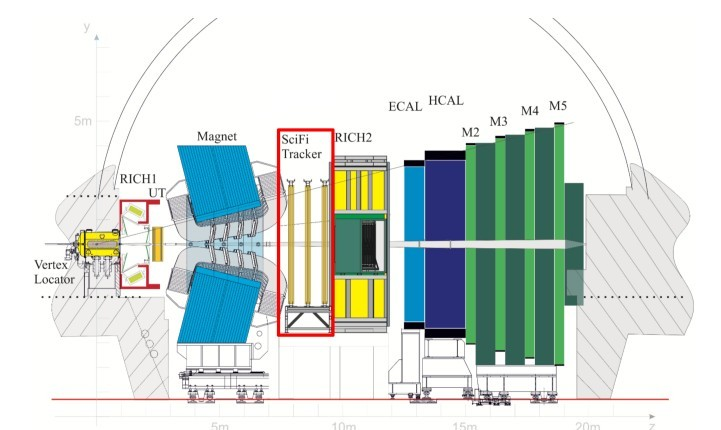
\includegraphics[width=0.8\linewidth]{Figure/LHCb.jpg}
    \caption{Schematic overview of the LHCb detector in Run 3 \cite{lhcb}.}
    \end{figure}
    
    The LHCb detector tracks particles only in the forward direction - unlike the other major detectors at CERN. The vertex locator finds both the primary and the  secondary vertices of the p-p collisions, while two RICHs (Ring Imaging CHerenkov Detector) measure the Cherenkov radiation angles, which in turn can be used to calculate the velocity of the particles.\\
    
    Moreover, the scintillating fiber tracker just after the magnet detects how much of the particle track is bent in the magnetic field. This helps in calculating the momentum of the particles. The mass of the particles can be easily extracted using the momentum and velocities. This helps in identifying particles except for high-energy muons.  
    
    \section{Scintillating Fibers}
    Scintillating fibers used in the LHCb SciFi Tracker consist of a $220~\mu m$ thick polystyrene core surrounded by two thin cladding layers, each $7.5~\mu m$ thick, giving a total diameter of $250~\mu m$. The fibers can achieve a resolution of less than $100~\mu m$. 

    \begin{tcolorbox}[colback=green!5!white,
                  colframe=green!60!black,
                  coltitle=white,
                  fontupper=\bfseries]
    
    This is only possible because of the \textbf{statistical distribution of the signal}. If the hit position is uniformly distributed over the fiber width \( w = 250~\mu m \), the variance or the spatial resolution is given by:

    \[
    \text{Var} = \frac{w^2}{12} = \frac{(250~\mu m)^2}{12} \approx (72~\mu m)^2
    \]

    So, the \textbf{position resolution} is approximately:

    \[
    \sigma = \sqrt{\text{Var}} \approx 72~\mu m
    \]
    
    \end{tcolorbox}

    % ?? %
    
    The core acts as the active scintillator medium, while the cladding provide the necessary refractive-index gradient to enable total internal reflection of the produced photons. Photons travel along the fiber by total internal reflection, primarily within the core. The efficiency of photon guidance is characterized by the capture angle, which is the maximum angle a photon can have relative to the fiber axis and still be totally internally reflected. Analytical expressions describe the path length 
    
    \begin{align}
        L = \frac{x}{\cos \theta}
    \end{align}
     and the number of reflections 
     
     \begin{align}
         N = \frac{x \tan \theta}{2\sqrt{r_{\text{core}}^2 - r_{\text{min}}^2}}
     \end{align} 
     with \(r_{\text{min}}\) being the minimal radial distance from the fiber axis. Although $r_{min}$ cannot be measured directly, simulations help estimate it. If $r_{min}=0$, then we get the simplified expression, achieving the maximum number of possible reflections in a fiber: 
     \begin{align}
         N = \frac{x \tan \theta}{2 r_{core}}
     \end{align}
    Photon energy losses inside the fiber occur via two main mechanisms: material attenuation (e.g., Rayleigh scattering, absorption by molecular vibrations or self-absorption) and reflection losses at the core-cladding interface. These losses are combined in a formula for the transmitted intensity 
    \begin{align}
        I(x, \theta) = I_0 \exp\left(-\frac{L}{\Lambda} - N \epsilon\right)
    \end{align} where $\Lambda$ is the attenuation length and $\epsilon$ the reflection loss per interface. The effective attenuation depends strongly on the photon's angle and path within the fiber, with minimal losses at zero angle. Together, these factors determine the light transport efficiency and performance of the scintillating fiber tracker, making this structure critical for precision tracking in the LHCb experiment.
    